\section{Durchführung}
\label{sec:Durchführung}

\begin{enumerate}
  \item  Es wird die Leerlaufspannung der Monozelle unmittelbar gemessen und
  der angegebene Eingangswiderstand $R_\text{V}$ notiert.

  \item  Die Klemmenspannung $U_\text{K}$ wird bei variablem Belastungsstrom $I$
  aufgenommen. Im Einzelnen werden 10 Messwertpaare aufgenommen.
  Um den Strom zu variieren wird  der Belastungswiderstand variiert.
  Das geschah durch Variation des variablen Widerstands im Bereich von 0-\SI{50}{\Omega}.
  Dazu wurde die Schaltung aus Abbildung \ref{fig:Schaltung1} verwendet.

\begin{figure}[h]
  \centering
  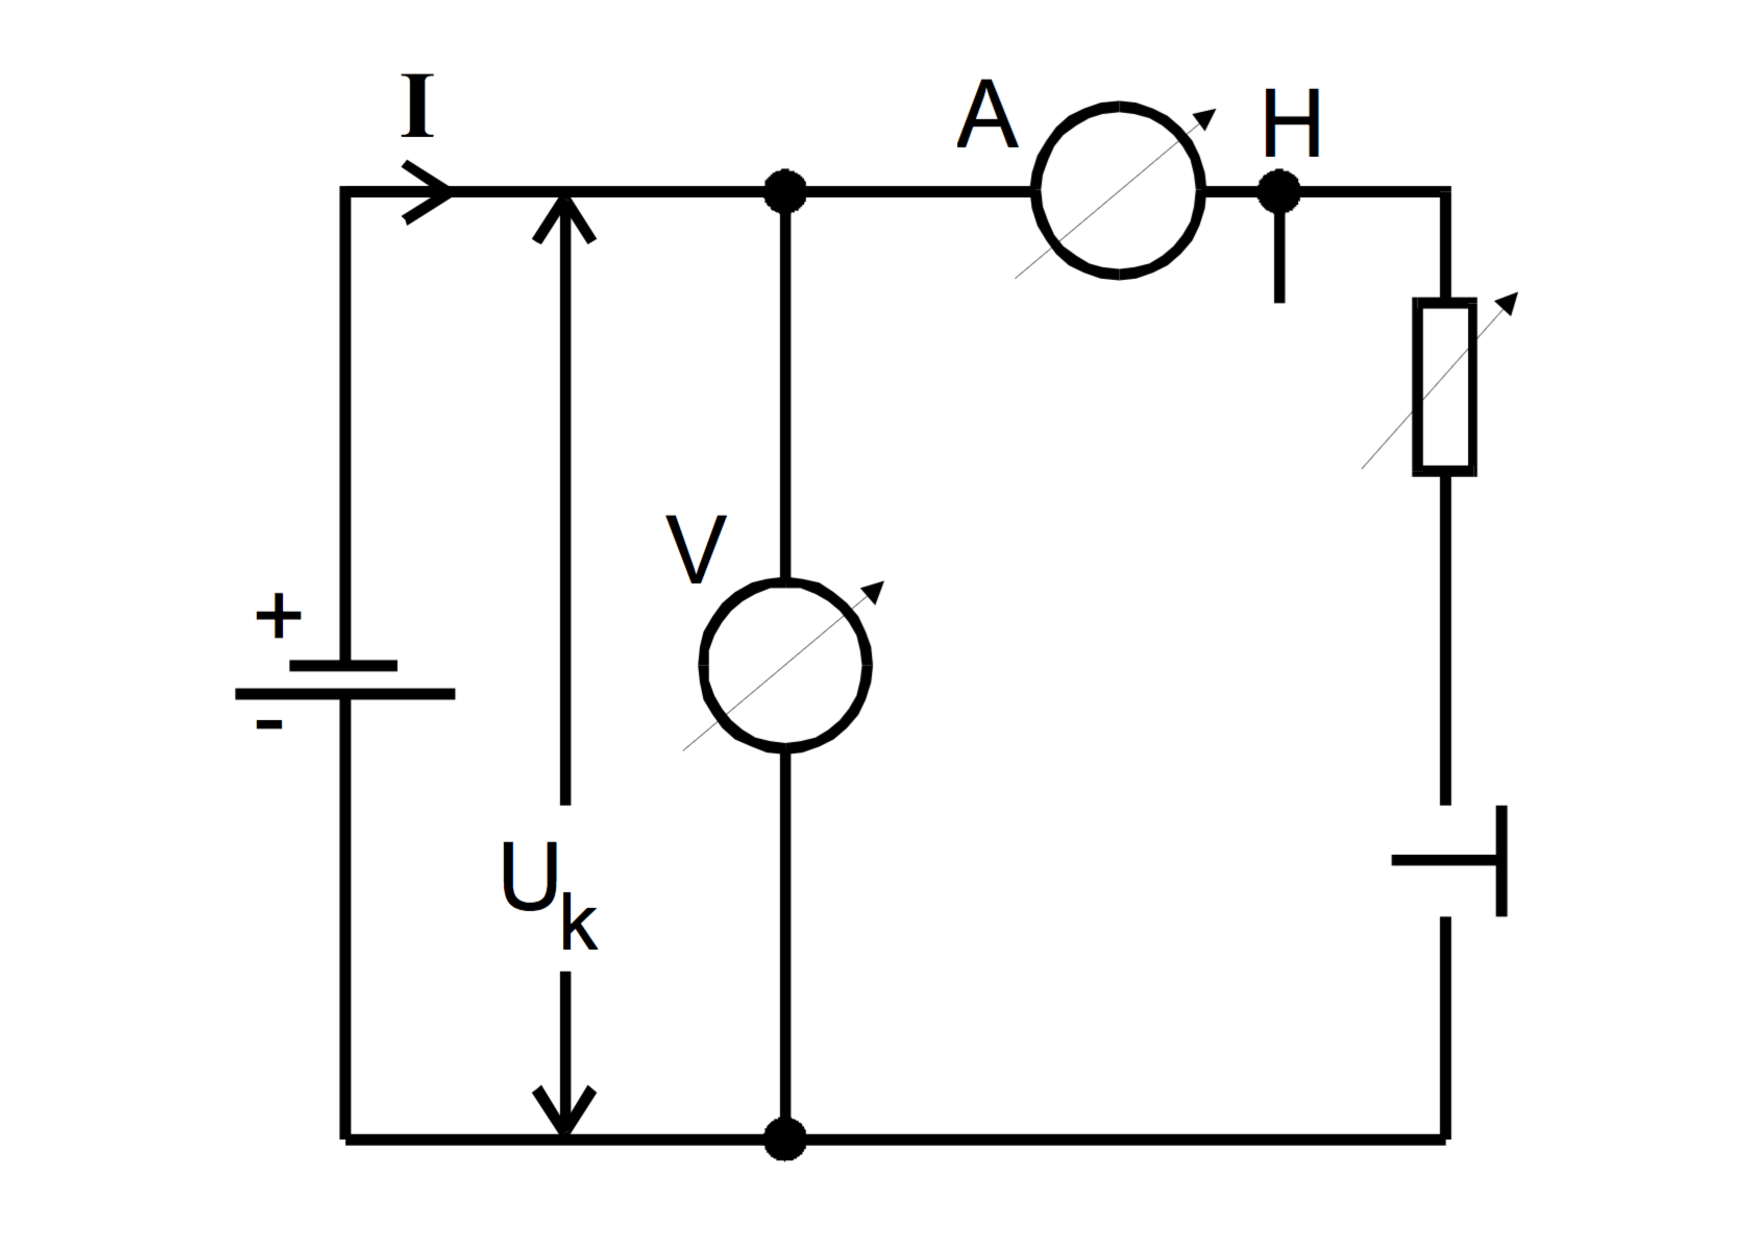
\includegraphics[height = 5cm]{Abbildung 1.pdf}
  \caption{Messschaltung 1 zum Messen an der Monozelle.\cite{anleitung}}
  \label{fig:Schaltung1}
\end{figure}

  \item Dann wird eine Gegenspannung in die Schaltung eingebaut, die den Strom
  in die entgegengesetzte Richtung fließen lässt, da sie ca. \SI{2}{\volt} größer
  ist als $U_{\text{0}}$. Hier ändert sich die Klemmenspannung
  wie in Gleichung \eqref{eqn:Gegenspannung}.

\begin{equation}
  U_\text{K} = U_\text{0} + IR_\text{i}
  \label{eqn:Gegenspannung}
\end{equation}

  Es wurden aber erneut $U_\text{K}$ und $I$ aufgenommen. Das geschah bei
  Variation des Widerstands im selben Bereich wie in Schritt 2. Es werden
  erneut 10 Messwertpaare notiert. Abbildung \ref{fig:Schaltung2}
  zeigt die verwendete Schaltung.

\begin{figure}[h]
  \centering
  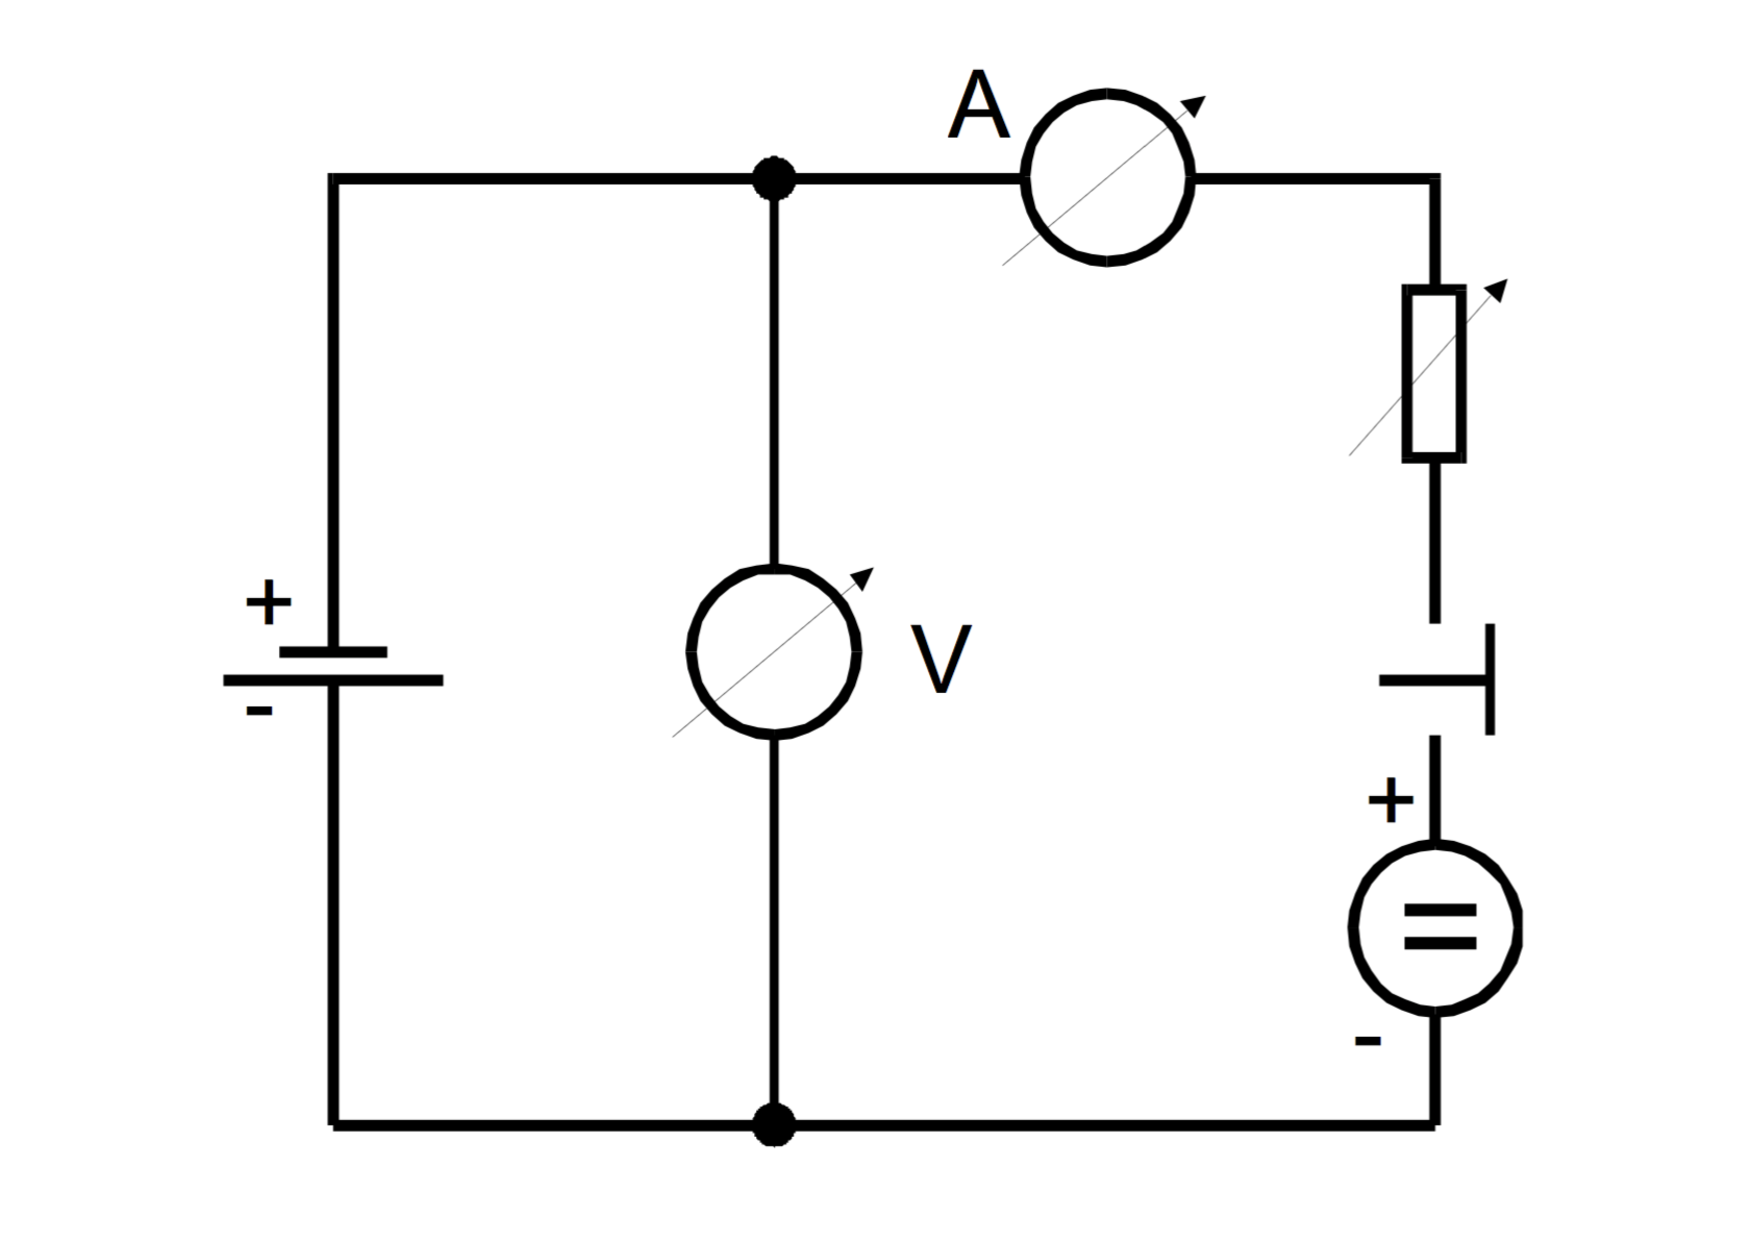
\includegraphics[height = 5cm]{Abbildung 2.pdf}
  \caption{Messschaltung 2 mit der Gegenspannung.\cite{anleitung}}
  \label{fig:Schaltung2}
\end{figure}

  \item Zuletzt wird die Messung aus Schritt 2 widerholt; allerdings mit dem Sinus-
  und Rechteckausgang eines RC-Generators als Messobjekt. $R_\text{a}$ wird für
  den \SI{1}{\volt}-Sinusausgang im Bereich von 20 bis \SI{250}{\Omega} und für den
  \SI{1}{\volt}-Rechteckausgang im Bereich von 0.1 bis \SI{5}{\kilo\Omega} variiert.
  Die Schaltungen mit dem Rechteck- und Sinusausgang als Messobjekte werden im
  Folgenden mit 3a beziehungsweise mit 3b bezeichnet. Sie sind analog zu Abbildung
  \ref{fig:Schaltung1} nur dass an Stelle der Gleichstromquelle der $RC$-Generator
  angeschlossen wird.
\end{enumerate}
